\documentclass[12pt]{article}
\usepackage{scrtime} % for \thistime (this package MUST be listed first!)
\usepackage[margin=0.75in]{geometry}
\usepackage{graphicx}
\usepackage{fancyhdr}
\usepackage{xspace}
%\usepackage{underscore}
\usepackage{pdfpages}
\usepackage{xcolor,colortbl}%for changing cell colour
\usepackage{longtable}
\usepackage{booktabs}
\pagestyle{fancy}
\setlength{\headheight}{15.2pt}
\setlength{\headsep}{13 pt}
\setlength{\parindent}{28 pt}
\setlength{\parskip}{12 pt}
\pagestyle{fancyplain}
\usepackage[T1]{fontenc}
\usepackage{tikz-cd}
\usepackage{tikz}
\usepackage[normalem]{ulem} %to strikeout text
\usetikzlibrary{decorations.markings}
\usetikzlibrary{calc, arrows}
\usepackage{lscape} %to make the page landscape
\usepackage{color,amsmath,amssymb,amsthm,mathrsfs,amsfonts,dsfont}
\usepackage{indentfirst} % to indent the first paragraph
\rhead{\fancyplain{}{Thesis Update \today \hfill Daniella Lato}}
%\rhead{\fancyplain{}{Thesis Update April 8, 2019 \hfill Daniella Lato}}
\title{Sinorhizobium Update}
\author{Daniella Lato}
\date{\today}
\renewcommand\headrulewidth{0.5mm}
\newcommand{\cc}{\cellcolor{black!16}}
\newcommand{\s}{\textit{Sinorhizobium}\xspace}
\newcommand{\smel}{\textit{S.\,meliloti}\xspace}
\newcommand{\smed}{\textit{S.\,medicae}\xspace}
\newcommand{\sfred}{\textit{S.\,fredii}\xspace}
\newcommand{\ssah}{\textit{S.\,saheli}\xspace}
\newcommand{\ster}{\textit{S.\,terangae}\xspace}
\newcommand{\agro}{\textit{A.\,tumefaciens}\xspace}
\newcommand{\escoli}{\textit{Escherichia coli}\xspace}
\newcommand{\bur}{\textit{Burkholderia}\xspace}
\newcommand{\vib}{\textit{Vibrio}\xspace}
\newcommand{\sul}{\textit{Sulfolobus}\xspace}
\newcommand{\ent}{\textit{Enterobacteria}\xspace}
\newcommand{\p}{progressiveMauve\xspace}
\newcommand{\bas}{\textit{Bacillus subtilis}\xspace}
\newcommand{\strep}{\textit{Streptomyces}\xspace}
\newcommand{\bass}{\textit{B.\,subtilis}\xspace}
\newcommand{\ecol}{\textit{E.\,coli}\xspace}
\newcommand{\ecoli}{\textit{Escherichia coli}\xspace}
\newcommand{\tub}{\textit{Mycobacterium tuberculosis}\xspace}
\newcommand{\pa}{pSymA\xspace}
\newcommand{\pb}{pSymB\xspace}
\newcommand{\snat}{\textit{S.\,natalensis}\xspace}
\newcommand{\scoe}{\textit{S.\,coelicolor}\xspace}
\newcommand{\borrb}{\textit{Borrelia burgdorferi}\xspace}
\providecommand{\e}[1]{\ensuremath{\times 10^{#1}}}
\newcommand{\ch}{$\checkmark$}
\newcommand{\dn}{\textit{dN}\xspace}
\newcommand{\ds}{\textit{dS}\xspace}
\newcommand{\sven}{\textit{S.\,venezuelae}\xspace}
%\newcommand{\scoe}{\textit{S.\,coelicolor}\xspace}
\newcommand{\sliv}{\textit{S.\,lividans}\xspace}
\begin{document}
%	Nov 30:	Create graphs with slopes for each COG
	
	
%	Dec 3:	Create new binned scatter plot of COG log reg
	
%	Dec 6:	Determine if there are any other stats I want/need for COG stuff
	
%	Dec 10:	Calculate above stats and write in table
	
%	Dec 21:	Find papers on COG stuff (for intro and discussion), and other mol trends (discussion for sub paper)
	
%	Jan 6:	Read above mentioned papers and make notes
%	Oct 31: Write out methods for gene expression paper
%	
%	Sep 9: Think about/compile list of inversions in \ecol for new paper
%	
%	Nov 15: Think about how to better look at the COG data
%	
%	Nov 25: Complete any extra analysis needed for Substitution paper
%	
%	Dec 4: Mac Scholarships and Awards Due
%	
%	Dec 1: Write out COG methods
%	
%	Dec 15: Gather papers for COG paper intro
%	
%	Dec 15: Implement COG stuff
%	
%	Other things to do:
%	
%	Create outline for gene expression paper
%
%  research mito increased subs near origin
%
%  add above to subs paper writeup
%	
%	Write Write Write gene expression paper
%	
%	 Have gene expression/inversion data combined and in graphical format/regression lines calculated
%	
%	re-do gene exp/sub graphs with patchwork R package so they line up exactly
%	
%	Have data for other molecular trends (GC content, number of genes, essential gene lists..etc.) combined with graphs (or in supplement) for sub analysis
%
% organize all the notes I made for comps into topics that can be integrated into an intro if needed
%	
%	May 31:	Complete COG analysis
%	
%	Jun 30:	COG analysis Paper draft completed
%	
%	Jul 31: Add other mol trends to Sub Paper

\underline{Subs Paper Things to Do:}
\begin{itemize}
%	\item \sout{ \# of coding and non-coding sites}
%	
%	\item \sout{\# of subs in each of $\uparrow$}
%	
%	\item \sout{Look into \strep non-coding issue}
%	
%	\item \sout{Look into \ecol coding issue}
%	
%	\item \sout{Look into \pb coding/non-coding trend weirdness}
%	
%	\item \sout{Figure out why \strep appears to have tons of coding data missing}
%	
%	\item \sout{Figure out what is going on with cod/non-cod code and why it is still not working!}
%	
%	\item \sout{write up methods for coding/non-coding}
%	
%	\item \sout{write methods and results for clustering}
%	
%	\item \sout{start code to split alignment into multiple alignments of each gene}
%	
%	\item \sout{figure out how to deal with overlapping genes}
%
%	\item \sout{figure out how to deal with gaps in gene of ref taxa}
%	
%	\item \sout{split up the alignment into multiple alignments of each gene}
%	
%	\item \sout{check if each gene alignment is a multiple of 3 (proper codon alignment)}
%	
%	\item \sout{get dN/dS for coding/non-coding stuff per gene}
%	 
%	\item Or get 1st, 2nd, 3rd codon pos log regs
	
%	\item \sout{write up coding/non-coding results}
%	
%	\item \sout{take out gene expression from this paper}
%	
%	\item \sout{write better intro/methods for distribution of subs graphs}
%	
%	\item \sout{write discussion for coding/non-coding}
%	
%	\item \sout{write coding/non-coding into conclusion}
%	
%	\item \sout{figured out pipeline for CODEML to calculate dN/dS for each gene}
%	
%	\item \sout{make a list of what should be in supplementary files for subs paper}
%	
%	\item \sout{put everything in list into supplementary file for subs paper}
%	
%	\item \sout{write dN/dS methods}
%	
%	\item \sout{write dN/dS results}
%	
%	\item \sout{write dN/dS discussion}
%	
%	\item \sout{write dN/dS into conclusion}
%	
%	\item \sout{new bar graph with coding and non-coding sites separated}
%	
%	\item \sout{spatial analysis of \dn, \ds, and $\omega$}

	\item causes for weird selection and subs results in \strep
	\begin{itemize}
		\item see how often class 4 arises in strep to see what is going on in later portion of the genome (to see if annotation is really a problem)
		
		\item split up the strep data into core and non core and see if results are the same
	\end{itemize}
	
	\item \sout{make graphs proportional to length of respective cod/non-cod regions}
	
	\item \sout{test examples for genes near and far from terminus (robust log reg/results)}
	
	\item \sout{linear regression on 10kb regions for weighted and non-weighted substitutions}
	
	\item \sout{average number of substitutions in 20kb regions near and far from the origin}
	
	\item \sout{figure out why the data is weird for number of cod/non-cod sites}
	
	\item why are the lin reg of \dn, \ds and $\omega$ NS but the subs graphs are...explain!
	
	\item grey out outliers in subs graphs?
	
	\item mol clock for my analysis?
	
	\item GC content? COG? where do these fit?
	
\end{itemize}

\underline{Gene Expression Paper Things to Do:}
\begin{itemize}
	
%	\item \sout{look for more GEO expression data for \smel}
%	
%	\item \sout{look for more GEO expression data for \strep}
%	
%	\item \sout{look for more GEO expression data for \bass}
%	
%	\item \sout{format paper and put in stuff that is already written}
%	
%	\item \sout{look for more GEO expression data for \ecol}
%	
%	\item \sout{Get numbers for how many different strains and multiples of each strain I have for gene expression}
%	
%	\item \sout{re-do gene expression analysis for \bass}
%	
%	\item \sout{re-do gene expression analysis for \ecol}
%	
%	\item \sout{find papers about what has been done with gene expression}
%	
%	\item \sout{read papers $\uparrow$}
%	
%	\item \sout{put notes from $\uparrow$ papers into word doc}
%	
%	\item \sout{write abstract}
%	
%	\item \sout{write intro}
%	
%	\item \sout{add stuff from outline to Data section}
%	
%	\item \sout{create graphs for expression distribution (no sub data)}
%	
%	\item \sout{add \# of genes to expression graphs (top)}
%	
%	\item \sout{average gene expression}
%	
%	\item \sout{write discussion}
%	
%	\item \sout{write conclusion}
%	
%	\item \sout{add into methods: filters for Hiseq, RT PCR and growth phases for data collection}
%	
	\item \sout{linear regression on 10kb regions}
	
	\item \sout{put new 10kb lin reg and \# of genes over 10kb lin reg into paper}
	
	\item \sout{write about $\uparrow$ in methods and discussion}
	
	\item \sout{put expression lin reg and \# coding sites log reg into supplement}
	
	\item \sout{write about $\uparrow$ in paper and how results are the same}
	
	\item \sout{update supplementary figures/file}
	
	\item \sout{correlation of gene expression across strains}
	\begin{itemize}
		\item \sout{make graphs pretty and more informative with label names}
		\item \sout{add them to supplement with a mini write up of what we did and why}
		\item \sout{mention this in the actual paper}
	\end{itemize}
	
	\item if necessary add a phylogenetic component to the analysis
	
	\item \sout{potentially remove genes that have been recently translocated from the analysis}
	
	\item \sout{model gene exp + position + number of genes}
	
	\item \sout{split up the strep data into core and non core and see if results are the same}
	
	\item \sout{what is going on with \strep number of genes changing drastically from core to non-core}
	
	\item codon bias?
	
	\item \sout{what is going on with really high gene expression bars}
	
	\item edit paper
	
	\item submit paper
	
\end{itemize}

\underline{Inversions and Gene Expression Letter Things to Do:}
\begin{itemize}
%	\item \sout{get as much GEO data as possible}
%	\item \sout{find papers about inversions and expression}
%	
%	\item \sout{see how many inversions I can identify in these strains of \ecoli with gene expression data}
%	
%	\item \sout{read papers about inversions}
%	
%	
	\item \sout{check if opposite strand in \p means an inversions (check visual matches the xmfa)}
	
	\item \sout{check if PARSNP and \p both identify the same inversions (check xmfa file)}
	\item create latex template for paper
	\item \sout{put notes from papers into doc}
	\item \sout{use large PARSNP alignment to identify inversions}
	\item confirm inversions with dot plot
	\item make dot plot of just gene presence and absence matrix (instead of each site) to see if this will go better
	\item look up inversions and small RNA's paper Marie was talking about at Committee meeting
	\item write outline for letter
	\item write Abstract
	\item write intro
	\item write methods
	\item compile tables (supplementary)
	\item write results
	\item write discussion
	\item write conclusion 
	\item do same ancestral/phylogenetic analysis that I did in the subs paper 
\end{itemize}

\underline{General Things to Do:}
\begin{itemize}
	\item summarize references 40 and 56 from Committee meeting report (Brian was asking)
	
	\item read and make notes on papers I found for dissertation intro
	
	
\end{itemize}


% next week look into how to calculate the dN/dS for the subs paper
% week of Dec 17th do same ancestral analysis on gene exp data for ecoli...which is going to require me to do everything from scratch so make a tree and all that jazz

	
\section*{Last Week}

\ch length cutoff for non-coding sections

\ch re-run subs analysis

\ch new graphs for gene expression data

\ch talked to Marie about \strep

\ch started selection analysis

\textbf{Subs analysis}
I re-did the analysis for the substitutions part of my thesis.
I had the results all laid out but my new laptop died so I didn't have time to put it all together here.
But as soon as I have the results together I will let you know!
From what I remember it looks roughly the same as before.
We decided to use the same cutoff for the non-coding sections (100bp) as for the coding sections.

I also made new gene expression graphs for all the bacteria which has a more efficient code, but also has \strep having negative numbers to make the graph clearer.
Again, once I get my laptop sorted I will show you these figures.
The only graph that was not working was the \smel chrom. 

\textbf{Talk with Marie}
I spoke with Marie about the \strep and she suggested as an alternative solution to look at just the core genome of \strep.
There are a lot of papers that state that the core is similar but the terminal ends are just really out of wack. So she thinks it would not be too hard to justify.
She sent me some papers with other phylogenies of \strep so I am going to have a look at the to see if I can find any appropriate groupings with more genomes.

\textbf{Selection analysis}
I started to re-do this analysis with the incorporation of Gblocks, but have hit some snags.
Because these sequences need to begin with the start of a codon, and end with the end of a codon, I am having trouble making this happen.
Hopefully I can figure this out this week. 




%Last week I did linear regression on the total number of substitutions in 10kb sections of the genome as well as a proportional number of substitutions for protein coding and non-protein coding sites (Table \ref{tab:lin_reg_10kb_subs}).
%Mostly everything is not significant or negative which is good!
%The only weird thing is that \strep is positive in non-protein coding when looking at proportional number of substitutions, but is negative when looking at raw counts of substitutions.
%I did a linear regression on the number of protein coding and non-protein coding sites and there is a significant negative correlation between the number of sites and distance from the origin of replication.
%So I think that there are just less sites here so that is why the proportion of substitutions per site increases near the end, but the raw number of substitutions is low.
%I will come discuss this with you later.

%I also calculated an average number of substitutions in 20kb regions near and far from the origin, these are found in Table \ref{tab:20kb_near_far_ori}.
%The origin does have a higher number of substitutions near the origin than compared to the terminus, which is great!
%However, the number of substitutions is higher in protein coding regions than in non-protein coding regions.
%I also wrote a little script to check if the proportional number of substitutions was higher in each 10kb region for non-protein coding v.s. protein coding, and I found the opposite.
%That the proportional number of substitutions (number of subs divided by number of sites) is higher in protein coding than non-protein coding in 60\% of the \ecol 10kb regions.
%I am still looking into this, I think that it may be something wrong with how I split up the alignments into protein coding and non-protein coding.
%So I need to look at this code carefully.
%%%%%%%%%%%%%%%%%%%%%%%%%%%%%%%%%%%%%%%%%%%%%%%%%%%%%%%%%%%%%%%%%%

%\textbf{dN, dS, $\omega$:}

%For the \dn, \ds results (Table \ref{tab:dN_dS_ratios}) we see that for all the replicons that have $\omega$ < 1, \dn < \ds, as it should be.
%The only replicon that has and $\omega$ > 1 is \strep and it has \dn > \ds, also as it should be.
%So, using the classic definition of what it means to have $\omega$ > 1, the mutations here are going through positive selection which kind of makes sense because for \strep we are looking at different SPECIES so they are collectively trying to gain an advantage.
%Where as for the other bacteria, $\omega$ < 1 suggests that most of the sites are going through purifying selection and therefore removing deleterious mutations. Which again kind of makes sense because here we are looking at the same SPECIES, in a variety of strains so they should be now trying to streamline their genome by removing bad things instead of trying to gain advantageous mutations.
%What are your thoughts on this?

%Finally the re-running of the selection and substitution analysis has finished! The results are found in the graphs and tables below.
%The new logistic regression for the substitution analysis looks like now only \bass and \smel Chromosome and \pa have a decreasing trend. The %other replicons have a positive trend. So it is pretty evenly split with 3 positive replicons and 3 negative replicons.
%Thoughts?
%I also re-did the coding/non-coding substitutions histograms and they look way nicer now! (See below)
%The only thing that is weird is that \strep has a positive linear regression for both coding and non-coding, but the graph looks negative...
%
%I also quickly fit linear regression models to the \dn, \ds, and $\omega$ values as they vary across the genome (Table \ref{tab:dN_dS_lin_reg}).
%As you can see, mostly nothing is significant. I think this is because most of the graphs are very non-linear and are quite spiky/variable throughout the genome.
%When looking at the graphs of the distribution of \dn, \ds, and $\omega$ they are quite spiky and not very pretty. Not sure if they are informative.
%Three weird things about this is that \ecoli, \bass and \pa appear to have chunks of data missing from their genomes. 
%When you look at the substitutions graphs you can see that there are less substitutions total in those areas, so it could just be a lack of data.
%I am looking into this more.
%
%When comparing the average genome \dn, \ds, and $\omega$ values to the violin plots, you can see that half of the replicons have $\omega$ values $>$ 1, but the corresponding violin plot shows that the median $\omega$ value is $<$ 1 except for \strep. So I am not sure if it is better to use the median or average vale?
%
%That being said, \strep still has \dn $>$ \ds. So the errors I found before did not fix this. I will continue to look into this.
%
%Dotter takes a few days to run (which is not ideal), but I have played with the window size in the hopes to reduce some of the noise.
%However, when looking at my original dot plot compared to the one you produced in mummer, they look different.
%Mine looks like there are at least 3 inversions total near the beginning and ends of the genome (I will have to show you on my computer because it takes way too long to load).
%And yours looks like there are no inversions at all..which is curious.
%Any thoughts on this?
%
%I also calculated the average gene expression per replicon for fun, this is found in Table \ref{tab:gene_exp_mean}. \strep is like 2 orders of magnitude lower than everything else..which is weird so I am not sure what is going on there.
%Do you think this is something that needs to be put into the gene expression paper?


%I have also been working to put the \dn, \ds, and $\omega$ values for each gene into a supplementary table on github. This is slowly getting done.



%\begin{itemize}
%	\item Is 5 genomes going to provide enough data/information?
%	\item would I use a midpoint for each gene and have one data point per node in the tree per gene?
%	\item or should I have all positions in the gene have the same expression value?
%\end{itemize}

%For the papers solely on gene expression, they were all basically saying the things that we already know, that gene expression tends to decrease when moving away from the origin.
%However, there were varying explanations as to why this was happening. Some papers attributed this to an increase in gene dosage near the origin, but others said that this was not the case and there must be some other mechanism for controlling this or that gene expression trends could be a secondary effect of selection on say gene order or chromosome organization.
%But, they all basically said that because bacterial genomes are so highly organized based on gene order, physical folding of the chromosome, co-regulation of gene clusters...etc that this is why we see gene expression decreasing when moving away from the origin of replication.
%
%For the papers on Inversions, the results were a bit all over the place.
%Most of the papers were older (1980's) and often focused on one known inversion in one bacteria.
%These often were related to antibiotic resistance, flagella state of bacteria, or turning specific genes on/off.
%Sometimes these studies would say how the inversion altered expression of close down or upstream genes by changing promoters locations.
%Other studies engineered their own inversions, some mentioning gene expression and some don't and talk more about the replication of inversions or how they tend to be symmetrical around the origin.
%One large study done with Staphylococcus in 2012 just mentions that lots of genes are deferentially expressed (some up regulated and some down regulated).
%The overall feeling I got was that inversions can alter gene expression and this can be done by changing the promoter location of specific genes, which can impact many things about the bacteria like their growth state and resistance.
%There seems to be no ``trend'' with respect to inversions always causing gene expression to go up or down.
%It also looks like no one has done what we are doing: looking at existing expression data to see how having an inversion impacts gene expression within and outside of the inversion.

%I also looked at the inversions and gene expression for the 5 strains of \ecol and there are inversions (pics of alignments below, the taxa with all the weird stuff going on is ATCC)!!
%Mauve identified 3 large inversions roughly: 1,000,000bp, 800,000bp and 500,000bp. 
%Parsnp identified similar inversions (in similar locations) roughly: 1,350,000bp, 547,000bp and 1,376,300bp.
%Both of the programs had some sections that were not within an LCB or part of the core genome within these regions so the actual continuous length of the inversions may be smaller.
%These inversions only exist in one of the bacteria: \ecoli ATCC. The other 4 strains are all VERY similar with hardly any rearrangements, let alone inversions.
%So based on this we decided that we can just compaire the inversions between K-12 MG1655 and ATCC.
%I believe that \p is only showing information from one strand so when something is listed on the opposite strand from the reference in \p then it should be an inversion. I obviously need to check this and make sure this is the case. If it is, then it will make coding to identify inversions super simple!
%Also need to check if the inversions identified by \p and PARSNP are the same.

%%%%%%%%%%%%%%%%%bring these up next time!!!

%I realized that for \pb I miscalculated the bidirectionality transformation, so I had to fix this and re-run everything.
%It did not change the logistic regression results (seen below).
%However, when I re-did the origin shuffling to see if the placement of the origin changed anything, moving the origin 100kb, 90kb and 80kb to the left made the logistic regression negative (opposite). I have been trying to figure out why this is happening but I am having no luck. I thought maybe it was because these shufflings are now ~700kb away from the terminus, but the actual origin is about the same distance. I am still trying to figure this out but I am not sure what to do or what it means about the robustness of the origin shuffling.

%I looked at the gene expression data for \smel in detail and it appears to look ok.
%When I graph the raw data and plot the regression line it looks like there is no trend for \smel, the points are evenly distributed throughout the genome and there appears to be no increasing or decreasing trend.
%When looking at the other bacteria's raw data, there is clearly a decreasing trend when moving away from the origin.
%Additionally the number of genes and number of replicates are all comparable between \smel and the other bacteria.
%So I think that the reason \smel does not have significant gene expression regressions is because there is simply no trend.

%Last week I was reading an average of 2 articles a day (and will continue to do so until Aug 15). 
%While reading these papers I was researching the increased number of substitutions found near the origin of mitochondria.
%The papers I found on this subject are slightly misleading. The titles suggest that the substitution rate near the Control Region (CR) of mitochondria (which spans the origin on either side) is higher.
%However, after reading the articles I found that the substitution rate is higher than what was previously estimated using phylogenetic methods.
%So, I need to do a bit more research to see if I can find what the substitution rate for the rest of the mt genome is and see if the CR actually is higher.

\section*{This Week}
%aim to tick off 4 tasks a week
%
Substitutions project:
\begin{enumerate}
	\item get new tree picture for ne \strep genomes
	\item figure out issue with alignment length for selection analysis
	\item re-run selection analysis
	\item figure out why \smel chromosome gene expression graph is not working
\end{enumerate}


\section*{Next Week}
Gene Expression:
\begin{enumerate}
	\item new graphs for substitutions? (negative positions), write new (and better) code for this
	\item  look into journal requirements for submission
	\item write cover letter for gene expression paper
	\item substitutions paper edits
\end{enumerate}

\newpage
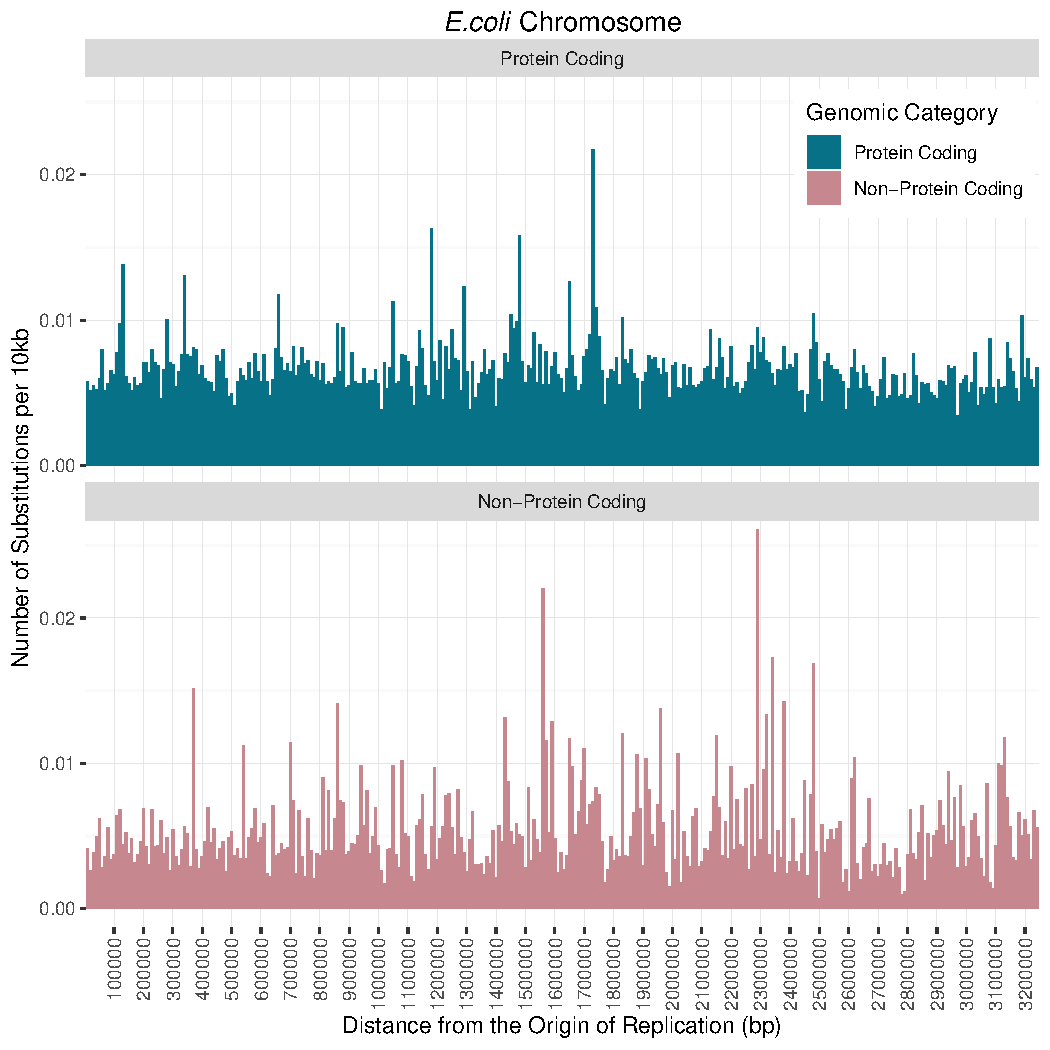
\includegraphics[width=\textwidth]{ecoli_chrom_cod_non_cod_weighted_sub_histogram_bidirectionality_colour_24Oct19.pdf}
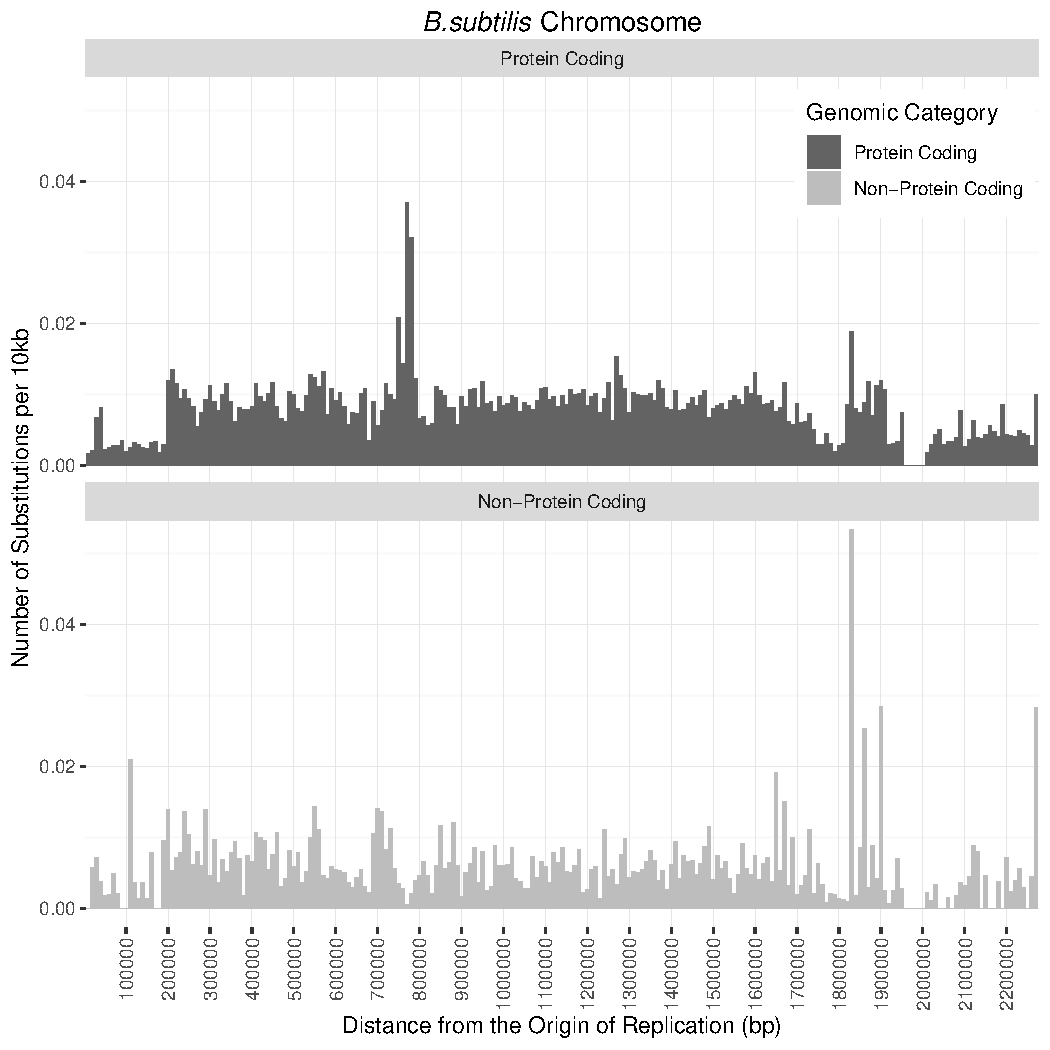
\includegraphics[width=\textwidth]{bass_chrom_cod_non_cod_weighted_sub_histogram_bidirectionality_colour_23Oct19.pdf}
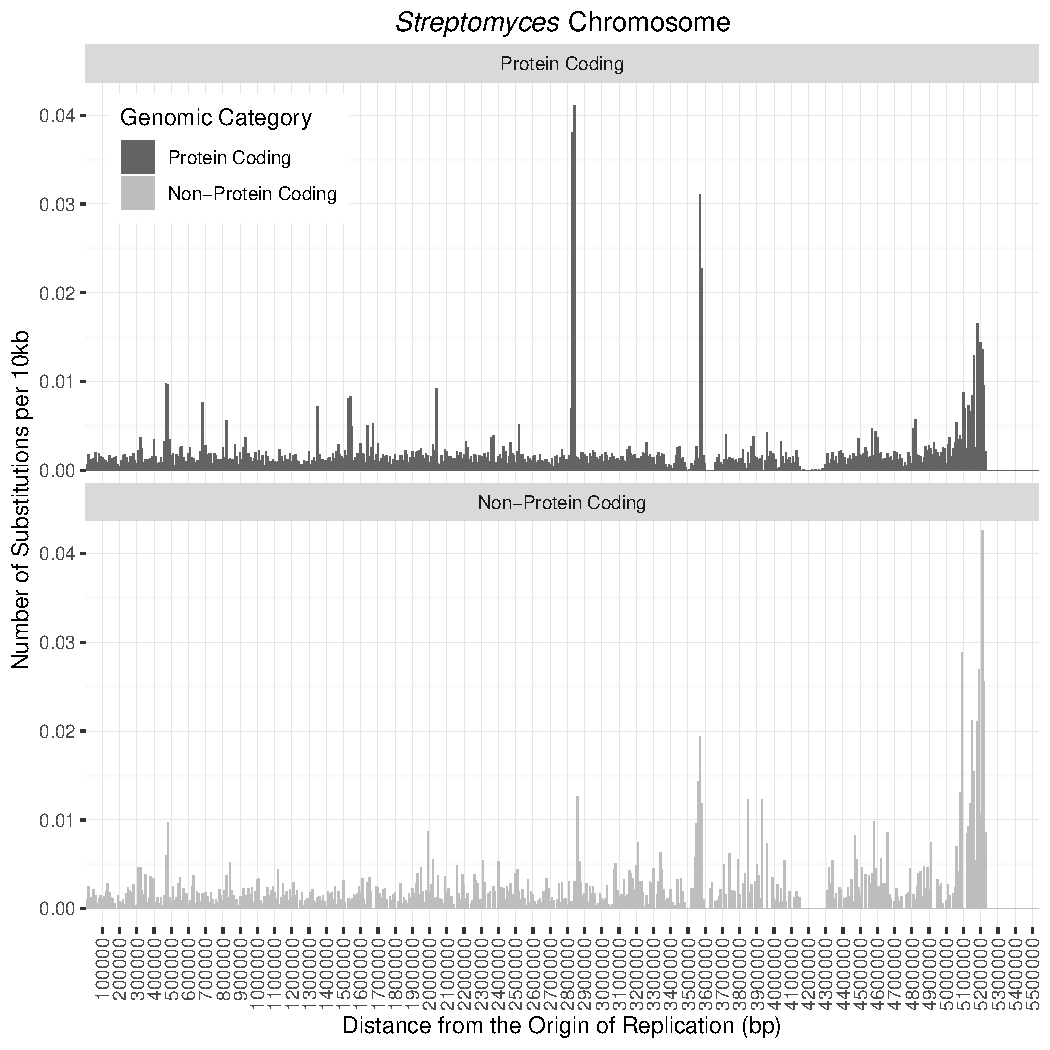
\includegraphics[width=\textwidth]{strep_chrom_cod_non_cod_weighted_sub_histogram_bidirectionality_colour_28Oct19.pdf}
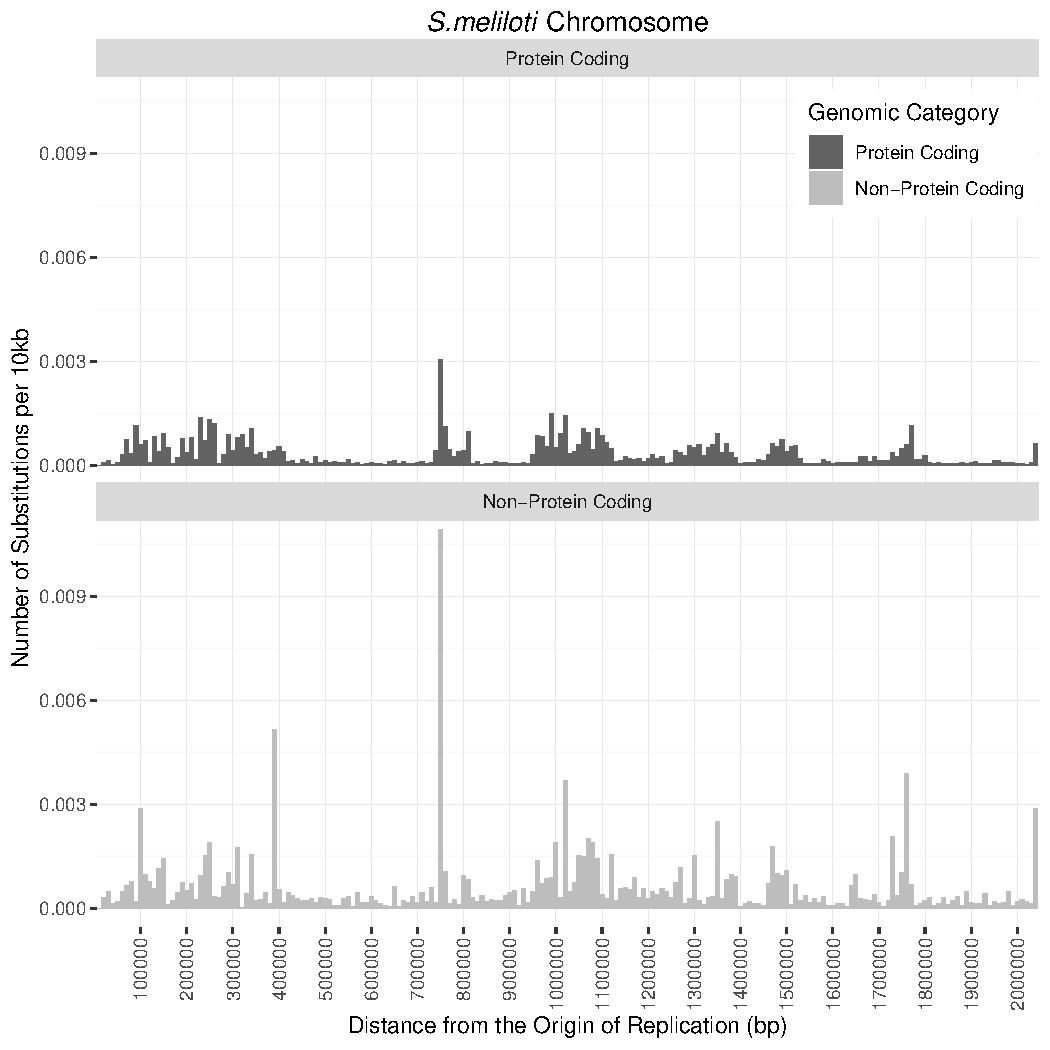
\includegraphics[width=\textwidth]{sinoC_chrom_cod_non_cod_weighted_sub_histogram_bidirectionality_colour_24Oct19.pdf}
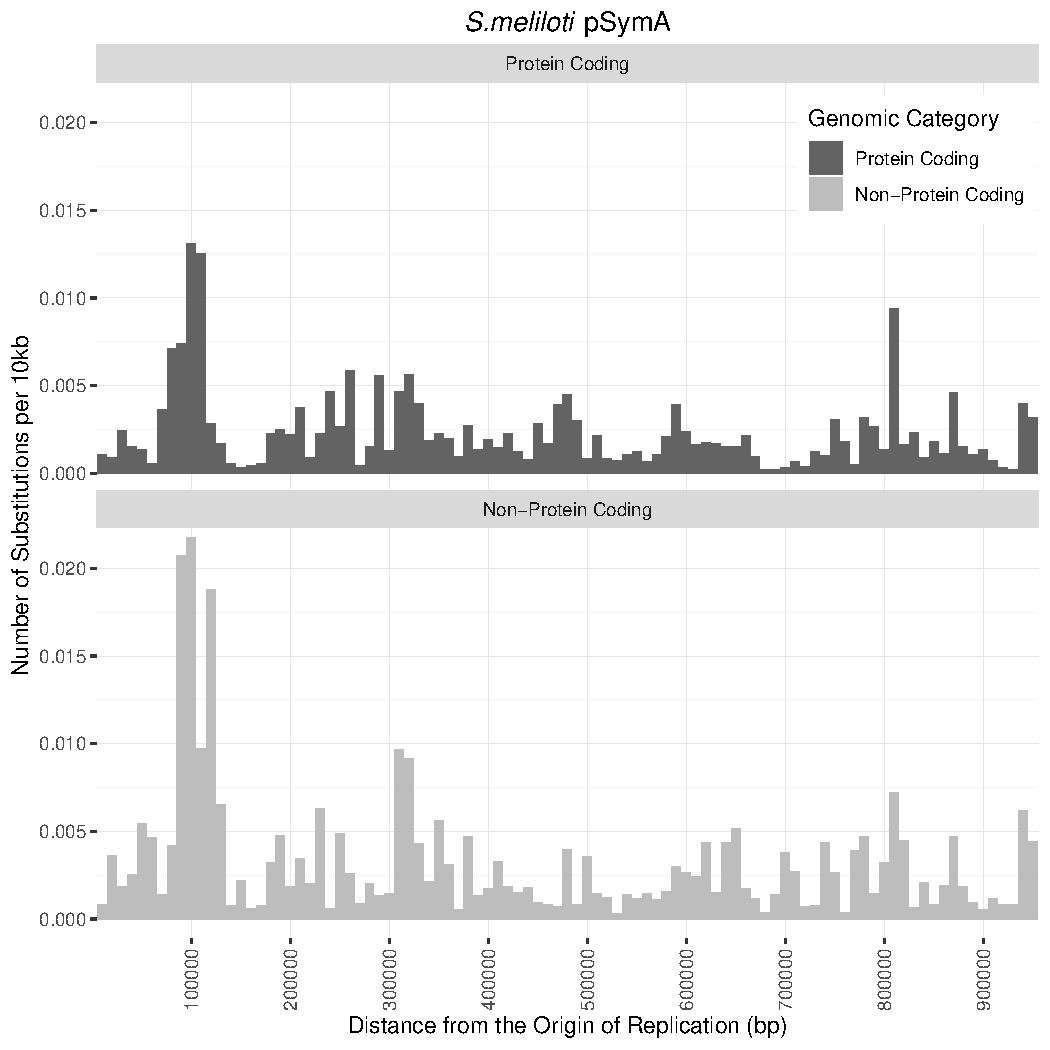
\includegraphics[width=\textwidth]{pSymA_chrom_cod_non_cod_weighted_sub_histogram_bidirectionality_colour_23Oct19.pdf}
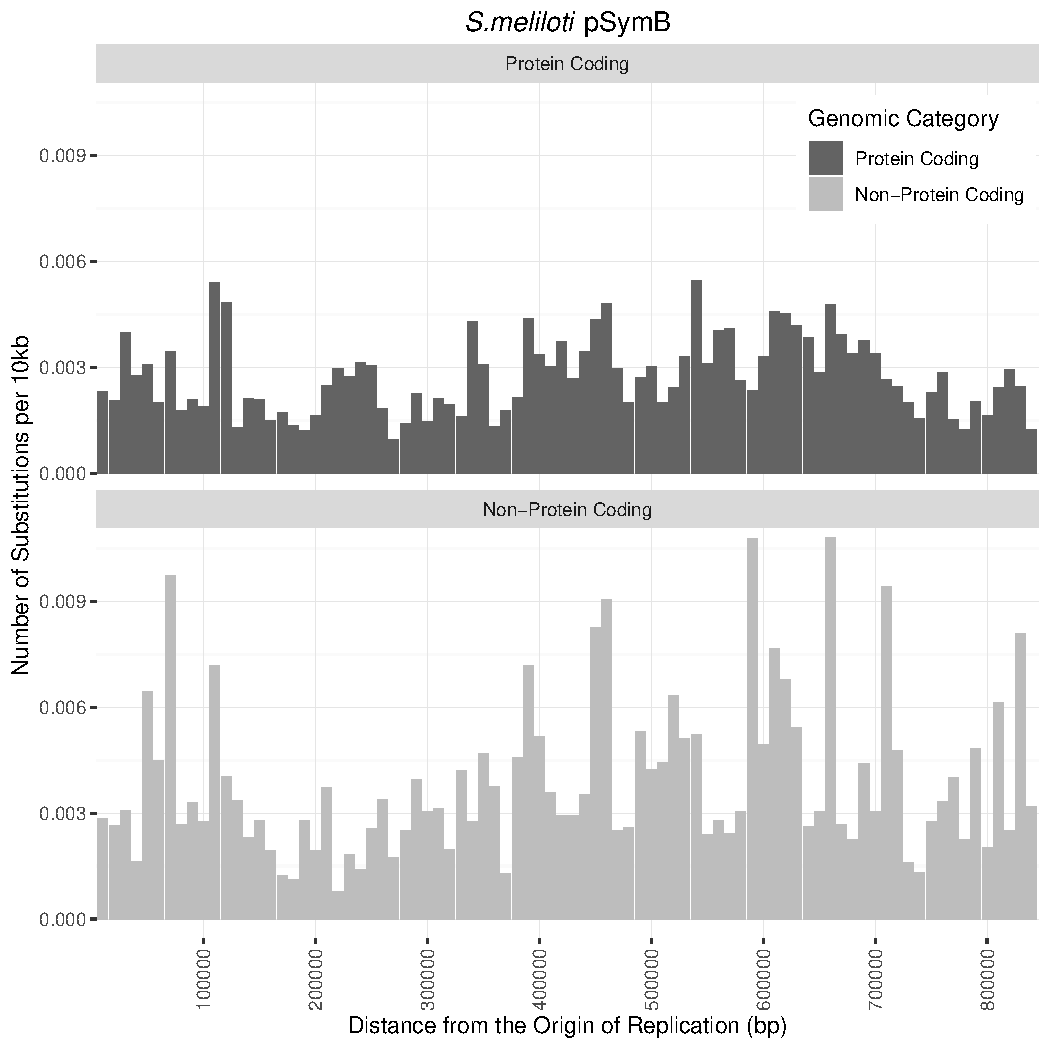
\includegraphics[width=\textwidth]{pSymB_chrom_cod_non_cod_weighted_sub_histogram_bidirectionality_colour_23Oct19.pdf}


%\begin{table}[h]
%	\centering
%	\resizebox{\textwidth}{!}{%
%		\begin{tabular}{lcrr}
%			\toprule
%			Bacteria and Replicon & Genomic Position (bp) & Protein/Gene Examples \\
%			\midrule
%			\ecol Chromosome & 0 - 10000 & DNA replication and repair\\
%			& & ATP-proton motive force\\
%			& & ATP biosynthesis\\
%			& & transport\\
%			& 470000 - 480000 & DNA replication and repair\\
%			& & tRNA synthesis\\
%			& & Ribosomal proteins\\
%			& & Putative transport\\
%			& 610000 - 620000 & Ribosomal protein\\
%			& & Translation modification\\
%			& & tRNA modification\\
%			& & RNA synthesis\\
%			\midrule
%			\bass Chromosome & 0 - 10000 & tRNA modification\\
%			& & Ribosomal proteins\\
%			& & DNA gyrase\\
%			& & rRNA small subunit methylation\\
%			& 130000 - 140000 & Ribosomal proteins\\
%			& & Elongation factor\\
%			& 730000 - 740000 & tRNA subunit\\
%			& & Transcription regulation\\
%			& & Glycolysis\\
%			& 1220000 - 1230000 & Pyruvate kinase\\
%			& & Sporulation membrane proteins \\
%			& & ATP-binding\\
%			& & Regulation protein\\
%			\midrule
%			\strep Chromosome & 1590000 - 1600000 & Ribosomal proteins\\
%			& & Hypothetical proteins\\
%			& 1690000 - 1700000 & Ribosomal proteins\\
%			\midrule
%			\smel Chromosome &  1480000 - 1490000 & Ribosomal proteins\\
%			& & Structural elements\\
%			& & Transmembrane proteins\\
%			\midrule
%			\smel pSymA & 660000 - 680000 & Hypothetical proteins\\
%			& & Unknown proteins\\
%			& & Small molecule metabolism \\
%			\midrule
%			\smel pSymB & 290000 - 300000 & Cell Division\\
%			& & Small molecule metabolism\\
%			& & Cell processes\\
%			& 800000 - 810000 & Small molecule metabolism\\
%			\bottomrule
%		\end{tabular}
%		
%	}%resizebox
%	\caption{\label{tab:high_exp_bars} Table of high median CPM (Counts per Million) gene expression over 10kb genomic regions for each bacterial replicon and the associated proteins/gene functions found in that region. The genomic position begins at the origin of replication and continues in both directions until the terminus of replication (bidirectional replication).}
%\end{table}
%
%
%
%
%
%\begin{table}[h]
%	\centering
%	\resizebox{\textwidth}{!}{%
%		\begin{tabular}{lccc}
%			\toprule
%			Bacteria and Replicon & Coefficient Estimate & Standard Error & P-value \\
%			\midrule
%		\ecol Chromosome & -5.29\e{-5} & 1.66\e{-5} & $<$2\e{-16}  \\
%			\bass Chromosome &  -9.8\e{-5} & 2.4\e{-5} & 6.2\e{-4}\\
%			\strep Chromosome & -1.307\e{-6} & 1.72\e{-7} & 1.3\e{-13}\\
%			\smel Chromosome & 8.81\e{-6} & 4.06\e{-5} & NS (8.3\e{-1})\\
%			\smel pSymA & 1.33\e{-3} & 4.3\e{-4} & 3\e{-3}\\
%			\smel pSymB & 9.55\e{-5} & 2.1\e{-4} & NS (7.5\e{-1})\\
%			\bottomrule
%		\end{tabular}
%		
%	}%resizebox
%	\caption{\label{tab:lr_normalized_exp} Linear regression analysis of normalized expression and distance from the origin of replication. The noramlized expression values were calculated by dividing the total counts per million expression value per 10kb section of the genome by the total number of genes in the respective 10kb section. Linear regression was calculated after the origin of replication was moved to the beginning of the genome and all subsequent positions were scaled around the origin accounting for bidirectionality of replication. NS indicates Not Significant at P $\le$ 0.05.}
%\end{table}
%
%
%
%
%\begin{table}[h]
%	\centering
%	\resizebox{\textwidth}{!}{%
%		\begin{tabular}{lccc|ccc}
%			\toprule
%			& \multicolumn{3}{c|}{Near Origin} & \multicolumn{3}{c}{Near Terminus} \\
%				\cmidrule{2-7}
%			Bacteria and Replicon &  \dn & \ds & $\omega$ &  \dn & \ds & $\omega$ \\
%			\midrule
%			\ecol Chromosome & NS & NS & NS& 
%								NS& NS& NS\\
%			\bass Chromosome & NS & NS &  NS&
%								NS& NS& NS \\
%			\strep Chromosome & --- & --- & ---&
%								---& ---& ---\\
%			\smel Chromosome & 3.77\e{-8}** & 3.54\e{-7}** & 1.23\e{-6}** &
%								 NS& NS& NS\\
%			\smel pSymA & NS & NS & 3.42\e{-5}*&
%							 NS& NS& NS\\
%			\smel pSymB & NS & NS & NS&
%						 -3.24\e{-7}**& 8.33\e{-6}***& NS\\
%			\bottomrule
%		\end{tabular}
%		
%	}%resizebox
%	\caption{\label{tab:dN_dS_20genes} Linear regression for \dn, \ds, and $\omega$ calculated for each bacterial replicon for the 20 genes closest and 20 genes farthest from the origin of replication. All results are marked with significance codes as followed: p: $<$ 0.001 = `***', 0.001 $<$ 0.01 = `**', 0.01 $<$ 0.05 = `*', $>$ 0.05 = `NS'.}
%\end{table}
%
%
%
%%subs density cod and non cod
%
%%\includegraphics[width=\textwidth]{C:/Users/Daniella/Documents/Sinorhizobium2015/Figs/Sub_graphs_cod_non_cod_7Feb19/ecoli_chrom_cod_non_cod_weighted_sub_histogram_bidirectionality_colour_19Sep19.pdf}
%
%\newpage
%
%%\includegraphics[width=\textwidth]{C:/Users/Daniella/Documents/Sinorhizobium2015/Figs/Sub_graphs_cod_non_cod_7Feb19/bass_chrom_cod_non_cod_weighted_sub_histogram_bidirectionality_colour_17Sep19.pdf}
%
%%\includegraphics[width=\textwidth]{C:/Users/Daniella/Documents/Sinorhizobium2015/Figs/Sub_graphs_cod_non_cod_7Feb19/strep_chrom_cod_non_cod_weighted_sub_histogram_bidirectionality_colour_9Sep19.pdf}
%
%%\includegraphics[width=\textwidth]{C:/Users/Daniella/Documents/Sinorhizobium2015/Figs/Sub_graphs_cod_non_cod_7Feb19/sinoC_chrom_cod_non_cod_weighted_sub_histogram_bidirectionality_colour_19Sep19.pdf}
%
%%\includegraphics[width=\textwidth]{C:/Users/Daniella/Documents/Sinorhizobium2015/Figs/Sub_graphs_cod_non_cod_7Feb19/pSymA_chrom_cod_non_cod_weighted_sub_histogram_bidirectionality_colour_17Sep19.pdf}
%
%%\includegraphics[width=\textwidth]{C:/Users/Daniella/Documents/Sinorhizobium2015/Figs/Sub_graphs_cod_non_cod_7Feb19/pSymB_chrom_cod_non_cod_weighted_sub_histogram_bidirectionality_colour_16Sep19.pdf}
%
%
\begin{table}[h]
	\centering
	\resizebox{\textwidth}{!}{%
		\begin{tabular}{lcc}
			\toprule
			Bacteria and Replicon & Protein Coding Sequences & Non-Protein Coding Sequences\\
			\midrule
			\ecol Chromosome & \cc -1.887\e{-8}*** & 6.462\e{-8}*** \\
			\bass Chromosome & \cc -7.200\e{-8}*** & \cc -1.296\e{-7}*** \\
			\strep Chromosome & 3.703\e{-8}*** & 1.775\e{-7}***\\
			\smel Chromosome & \cc -2.024\e{-7}***  & \cc -1.594\e{-7}** \\
			\smel pSymA & \cc -5.894\e{-7}*** & \cc -6.904\e{-7}*** \\
			\smel pSymB & 1.361\e{-7}*** & 4.475\e{-7}***\\
			\bottomrule
		\end{tabular}
		
	}%resizebox
	\caption{\label{tab:cod_non_cod_log_reg} Logistic regression analysis of the number of substitutions along all positions of the genome of the respective bacteria replicons. These genomic positions were split up into the coding and non-coding regions of the genome. Grey coloured boxes indicate a negative logistic regression coefficient estimate. All results are statistically significant. Logistic regression was calculated after the origin of replication was moved to the beginning of the genome and all subsequent positions were scaled around the origin accounting for bidirectionality of replication. All results are marked with significance codes as followed: $<$ 0.001 = `***', 0.001 $<$ 0.01 = `**', 0.01 $<$ 0.05 = `*', $>$ 0.05 = `NS'.}
\end{table}




\begin{table}[h]
	\centering
	\resizebox{\textwidth}{!}{%
		\begin{tabular}{lcc|cc|cc|cc}
			\toprule
			& \multicolumn{4}{c|}{Protein Coding} &\multicolumn{4}{c}{Non-Protein Coding} \\
			\cmidrule{2-9}
			%			\cmidrule{8-10}
			%			& \multicolumn{3}{c}{Weighted} & \multicolumn{3}{c}{Non-weighted} & \multicolumn{3}{c}{Weighted} \\
			%			\cmidrule{2-3}
			%			\cmidrule{4-7}
			& \multicolumn{2}{c|}{Correlation Coefficient} & \multicolumn{2}{c|}{Number of Substitutions} & \multicolumn{2}{c|}{Correlation Coefficient} & \multicolumn{2}{c}{Number of Substitutions} \\
			& \multicolumn{2}{c|}{20kb Near} &\multicolumn{2}{c|}{per 20kb Near} & \multicolumn{2}{c|}{20kb Near} & \multicolumn{2}{c}{per 20kb Near}\\
			\cmidrule{2-9}
			Bacteria and Replicon &  Origin & Terminus& Origin & Terminus& Origin & Terminus & Origin & Terminus\\
			\midrule
			\ecol Chromosome &  \cc -1.343\e{-5}** & NS & 5.45\e{-3} & 6.60\e{-3}& NS & \cc -9.231\e{-5}** & 2.95\e{-3} & 4.67\e{-3} \\
			\bass Chromosome & NS & 3.114\e{-5}*** & 1.24\e{-3} & 8.00\e{-3} & NS & 7.906\e{-5}* & 1.35\e{-3}& 1.74\e{-2}\\
			\strep Chromosome & 9.938\e{-5}*** & \cc -8.242\e{-5}*** & 1.22\e{-3} & 7.77\e{-3} & NS & \cc -1.023\e{-4}*** & 1.66\e{-3} & 2.14\e{-2}\\
			\smel Chromosome & NS & NS & 9.45\e{-5} & 4.25\e{-5}& NS & NS & 1.61\e{-4} & 1.41\e{-4}\\
			\smel pSymA & NS & NS & 9.78\e{-4} & 6.89\e{-4} & 1.431\e{-4}** & NS & 2.51\e{-3}  & 9.44\e{-4} \\
			\smel pSymB & \cc -2.375\e{-5}*** & \cc -6.976\e{-5}*** & 2.18\e{-3} & 1.61\e{-3}  & NS & \cc -6.134\e{-5}** & 2.64\e{-3} & 5.23\e{-3}\\
			\bottomrule
		\end{tabular}
		
	}%resizebox
	\caption{\label{tab:20kb_near_far_ori} Logistic regression on 20kb closest and farthest from the origin of replication after accounting for bidirectional replication and outliers. All results are marked with significance codes as followed: $<$ 0.001 = `***', 0.001 $<$ 0.01 = `**', 0.01 $<$ 0.05 = `*', $>$ 0.05 = `NS'.}
\end{table}


\begin{table}[h]
	\centering
	\resizebox{\textwidth}{!}{%
		\begin{tabular}{lcc|cc}
			\toprule
			& \multicolumn{2}{c|}{Protein Coding} &\multicolumn{2}{c}{Non-Protein Coding} \\
			\cmidrule{2-5}
			Bacteria and Replicon &  Weighted & Non-Weighted & Weighted & Non-Weighted\\
			\midrule
			\ecol Chromosome & \cc -2.91\e{-10}*  & \cc -1.57\e{-4}***& NS & \cc -9.29\e{-6}***\\
			\bass Chromosome & \cc -1.150\e{-9}** & \cc -1.993\e{-4}** & NS & \cc -8.24\e{-6}** \\
			\strep Chromosome & NS & \cc -8.98\e{-6}***& 3.87\e{-10}*** & \cc -1.065\e{-6}*** \\
			\smel Chromosome &\cc -1.389\e{-10}** &\cc -1.425\e{-5}**& NS & NS\\
			\smel pSymA & \cc -2.01\e{-9}* & \cc -1.06\e{-4}* & \cc -3.95\e{-9}**& NS\\
			\smel pSymB & NS & NS & NS & NS\\
			\bottomrule
		\end{tabular}
		
	}%resizebox
	\caption{\label{tab:lin_reg_10kb_subs} Linear regression on 10kb sections of the genome with increasing distance from the origin of replication after accounting for bidirectional replication. Weighted columns have the total number of substitutions in each 10kb section of the genome divided by the total number of protein coding and non-protein coding sites in the genome. Non-weighted columns are performing a linear regression on the total number of substitutions in each 10kb section of the genome. All results are marked with significance codes as followed: $<$ 0.001 = `***', 0.001 $<$ 0.01 = `**', 0.01 $<$ 0.05 = `*', $>$ 0.05 = `NS'.}
\end{table}


\begin{table}[h]
	\centering
	\resizebox{\textwidth}{!}{%
	\begin{tabular}{lc}
			\toprule
			Bacteria and Replicon & Coefficient Estimate \\
			\midrule
			\ecol Chromosome & \cc -9.89\e{-8}***\\
			\bass Chromosome & \cc -2.239\e{-8}*** \\
			\strep Chromosome & \cc -8.23\e{-8}***\\
			\smel Chromosome & 1.265\e{-7}***\\
			\smel pSymA & 3.084\e{-7}888 \\
			\smel pSymB & \cc -2.172\e{-7}***\\
			\bottomrule
		\end{tabular}
		
	}%resizebox
	\caption{\label{tab:lr_gene_num} Linear regression analysis of the total number of protein coding genes per 10kb along the genome of the respective bacteria replicons. Linear regression was calculated after the origin of replication was moved to the beginning of the genome and all subsequent positions were scaled around the origin accounting for bidirectionality of replication. All results are marked with significance codes as followed: $<$ 0.001 = `***', 0.001 $<$ 0.01 = `**', 0.01 $<$ 0.05 = `*', $>$ 0.05 = `NS'.}
\end{table}



%\begin{table}[h]
%	\centering
%	\resizebox{\textwidth}{!}{%
%		\begin{tabular}{lc}
%			\toprule
%			Bacteria and Replicon & Gene Expression 10kb \\
%			\midrule
%			\ecol Chromosome & \cc -2.742\e{-5}**\\
%			\bass Chromosome & \cc -2.198\e{-5}*\\
%			\strep Chromosome & \cc -5.230\e{-7}*** \\
%			\smel Chromosome & NS\\
%			\smel pSymA & NS \\
%			\smel pSymB & NS \\
%			\bottomrule
%		\end{tabular}
%		
%	}%resizebox
%	\caption{\label{tab:lr_exp_10kb} Linear regression analysis of the median counts per million expression data for 10kb segments of the genome of the respective bacteria replicons. Linear regression was calculated after the origin of replication was moved to the beginning of the genome and all subsequent positions were scaled around the origin accounting for bidirectionality of replication. All results are marked with significance codes as followed: $<$ 0.001 = `***', 0.001 $<$ 0.01 = `**', 0.01 $<$ 0.05 = `*', $>$ 0.05 = `NS'.}
%\end{table}
%
%
%\begin{table}[h]
%	\centering
%	\resizebox{\textwidth}{!}{%
%		\begin{tabular}{lccc}
%			\toprule
%			Bacteria and Replicon & Coefficient Estimate & Standard Error & P-value \\
%			\midrule
%			\cellcolor{black!16}\ecol Chromosome & \cellcolor{black!16}-6.03\e{-5} & \cellcolor{black!16}1.28\e{-5} & \cellcolor{black!16}2.8\e{-6} \\
%			\cellcolor{black!16}\bass Chromosome & \cellcolor{black!16}-9.7\e{-5} & \cellcolor{black!16}2.0\e{-5} & \cellcolor{black!16}1.2\e{-6} \\
%			\cellcolor{black!16}\strep Chromosome & \cellcolor{black!16}-1.17\e{-6} & \cellcolor{black!16}1.04\e{-7} & \cellcolor{black!16}$<$2\e{-16}\\
%			\smel Chromosome & 3.97\e{-5} & 4.25\e{-5} & NS (3.5\e{-1})\\
%			\smel pSymA & 1.39\e{-3} & 2.53\e{-4} & 4.9\e{-8} \\
%			\smel pSymB & 1.46\e{-4} & 2.03\e{-4} & NS (5.34.7\e{-1})\\
%			\bottomrule
%		\end{tabular}
%		
%	}%resizebox
%	\caption{\label{tab:lr_exp} Linear regression analysis of the median counts per million expression data along the genome of the respective bacteria replicons. Linear regression was calculated after the origin of replication was moved to the beginning of the genome and all subsequent positions were scaled around the origin accounting for bidirectionality of replication.}
%\end{table}
%
%%\begin{centering}
%%	\includegraphics[width=\textwidth]{C:/Users/Daniella/Documents/Sinorhizobium2015/Gene_Expression_8Dec17/Gene_Expression/Graphs/ecoli_chrom_exp_tot_gene_num_bidirectionality_colour_5Jun19.pdf}
%%\end{centering}
%
%
%
%
%
%\begin{table}[h]
%	\centering
%	\resizebox{\textwidth}{!}{%
%		\begin{tabular}{lccc}
%			\toprule
%			Bacteria and Replicon &  \dn & \ds & $\omega$ \\
%			\midrule
%			\ecol Chromosome & NS & NS & NS\\
%			\bass Chromosome & NS & NS & \cc -9.08\e{-6}*\\
%			\strep Chromosome & NS & NS & NS\\
%            \smel Chromoeom & NS & NS & NS \\
%			\smel pSymA & NS & NS & NS\\
%			\smel pSymB & NS & NS & 1.163\e{-5}*\\
%			\bottomrule
%		\end{tabular}
%		
%	}%resizebox
%	\caption{\label{tab:dN_dS_lin_reg} Linear regression for \dn, \ds, and $\omega$ calculated for each bacterial replicon on a per genome basis. All results are marked with significance codes as followed: p: $<$ 0.001 = `***', 0.001 $<$ 0.01 = `**', 0.01 $<$ 0.05 = `*', $>$ 0.05 = `NS'.}
%\end{table}
%
%
%
%
%
%\begin{table}[h]
%	\centering
%	\resizebox{\textwidth}{!}{%
%		\begin{tabular}{lr}
%			\toprule
%			Bacteria and Replicon & Average Expression Value (CPM)\\
%			\midrule
%			\ecol Chromosome & 160.500\\
%			\bass Chromosome &  176.400\\
%			\strep Chromosome &  6.084\\
%			\smel Chromosome &  271.400\\
%			\smel pSymA & 690.100\\
%			\smel pSymB & 595.700\\
%			\bottomrule
%		\end{tabular}
%		
%	}%resizebox
%	\caption{\label{tab:gene_exp_mean} Arithmetic gene expression calculated across all genes in each replicon. Expression values are represented in Counts Per Million.}
%\end{table}
%
%\begin{table}[h]
%	\centering
%	\resizebox{\textwidth}{!}{%
%		\begin{tabular}{lrrrrrr}
%			\toprule
%			& \multicolumn{3}{c}{Gene Average} & \multicolumn{3}{c}{Genome Average}\\
%			\cmidrule{2-7}
%			%			\cmidrule{8-10}
%			%			& \multicolumn{3}{c}{Weighted} & \multicolumn{3}{c}{Non-weighted} & \multicolumn{3}{c}{Weighted} \\
%			%			\cmidrule{2-3}
%			%			\cmidrule{4-7}
%			Bacteria and Replicon &  dS & dN & $\omega$ & dS & dN & $\omega$ \\
%			\midrule
%			\ecol Chromosome & 1.0468 & 0.1330 & 1.3183 & 0.6491 & 0.0364 & 0.2432 \\
%			\bass Chromosome & 4.652 & 0.2333 & 2.4200 & 1.0879 & 0.0703 & 0.3852\\
%			\strep Chromosome &  13.4950 & 2.0973 & 21.0423 & 5.1256 & 0.8911  & 8.9146  \\
%			\smel Chromosome &  0.0184  & 0.0012 & 0.1069 & 0.0187 & 0.0013 & 0.0962 \\
%			\smel pSymA & 1.0602 & 0.7451 & 5.1290 & 0.4100 & 0.0863 & 0.8311 \\
%			\smel pSymB & 3.2602 & 0.0256& 0.3878& 0.1436 & 0.0100 & 0.1943\\
%			\bottomrule
%		\end{tabular}
%		
%	}%resizebox
%	\caption{\label{tab:dN_dS_ratios} Weighted averages calculated for each bacterial replicon on a per genome basis using the gene length as the weight. Arithmetic mean calculated for the per gene averages for each bacterial replicon.}
%\end{table}
% \newpage
%
%%Violin plots for per gene dN, dS, and $\omega$:
%%
%%\clearpage
%%
%%\includegraphics[width=\textwidth]{C:/Users/Daniella/Documents/Sinorhizobium2015/Figs/dN_dS_box_plots_15May19/ALL_BAC_dN_dS_omega_violinplots_11Jul19.pdf}
%%
%%\newpage
%%
%%\includegraphics[width=\textwidth]{C:/Users/Daniella/Documents/Sinorhizobium2015/Figs/dN_dS_omega_genome_distribution_24May19/ecoli_dN_dS_omega_dist_11Jul19.pdf}
%%
%%\newpage
%%
%%\includegraphics[width=\textwidth]{C:/Users/Daniella/Documents/Sinorhizobium2015/Figs/dN_dS_omega_genome_distribution_24May19/bass_dN_dS_omega_dist_11Jul19.pdf}
%%\newpage
%%
%%\includegraphics[width=\textwidth]{C:/Users/Daniella/Documents/Sinorhizobium2015/Figs/dN_dS_omega_genome_distribution_24May19/strep_dN_dS_omega_dist_11Jul19.pdf}
%%
%%\newpage
%%
%%\includegraphics[width=\textwidth]{C:/Users/Daniella/Documents/Sinorhizobium2015/Figs/dN_dS_omega_genome_distribution_24May19/sinoC_dN_dS_omega_dist_11Jul19.pdf}
%%
%%\newpage
%%
%%\includegraphics[width=\textwidth]{C:/Users/Daniella/Documents/Sinorhizobium2015/Figs/dN_dS_omega_genome_distribution_24May19/pSymA_dN_dS_omega_dist_11Jul19.pdf}
%%
%%\newpage
%%
%%\includegraphics[width=\textwidth]{C:/Users/Daniella/Documents/Sinorhizobium2015/Figs/dN_dS_omega_genome_distribution_24May19/pSymB_dN_dS_omega_dist_11Jul19.pdf}
%
%
%%
%%Gene expression graphs
%%
%%% Gene Exp graphs
%%\includegraphics[width=\textwidth]{C:/Users/Daniella/Documents/Sinorhizobium2015/Gene_Expression_8Dec17/Gene_Expression/Graphs/ecoli_chrom_sub_exp_histogram_bidirectionality_colour_13Mar19.pdf}
%%
%%\includegraphics[width=\textwidth]{C:/Users/Daniella/Documents/Sinorhizobium2015/Gene_Expression_8Dec17/Gene_Expression/Graphs/bass_chrom_sub_exp_histogram_bidirectionality_colour_4Mar19.pdf}
%%
%%\includegraphics[width=\textwidth]{C:/Users/Daniella/Documents/Sinorhizobium2015/Gene_Expression_8Dec17/Gene_Expression/Graphs/strep_chrom_sub_exp_histogram_bidirectionality_colour_4Mar19.pdf}
%%
%%\includegraphics[width=\textwidth]{C:/Users/Daniella/Documents/Sinorhizobium2015/Gene_Expression_8Dec17/Gene_Expression/Graphs/smel_chrom_sub_exp_histogram_bidirectionality_colour_4Mar19.pdf}
%%
%%\includegraphics[width=\textwidth]{C:/Users/Daniella/Documents/Sinorhizobium2015/Gene_Expression_8Dec17/Gene_Expression/Graphs/pSymA_sub_exp_histogram_bidirectionality_colour_4Mar19.pdf}
%%
%%\includegraphics[width=\textwidth]{C:/Users/Daniella/Documents/Sinorhizobium2015/Gene_Expression_8Dec17/Gene_Expression/Graphs/pSymB_sub_exp_histogram_bidirectionality_colour_4Mar19.pdf}
%%
%%
%%
%%
%%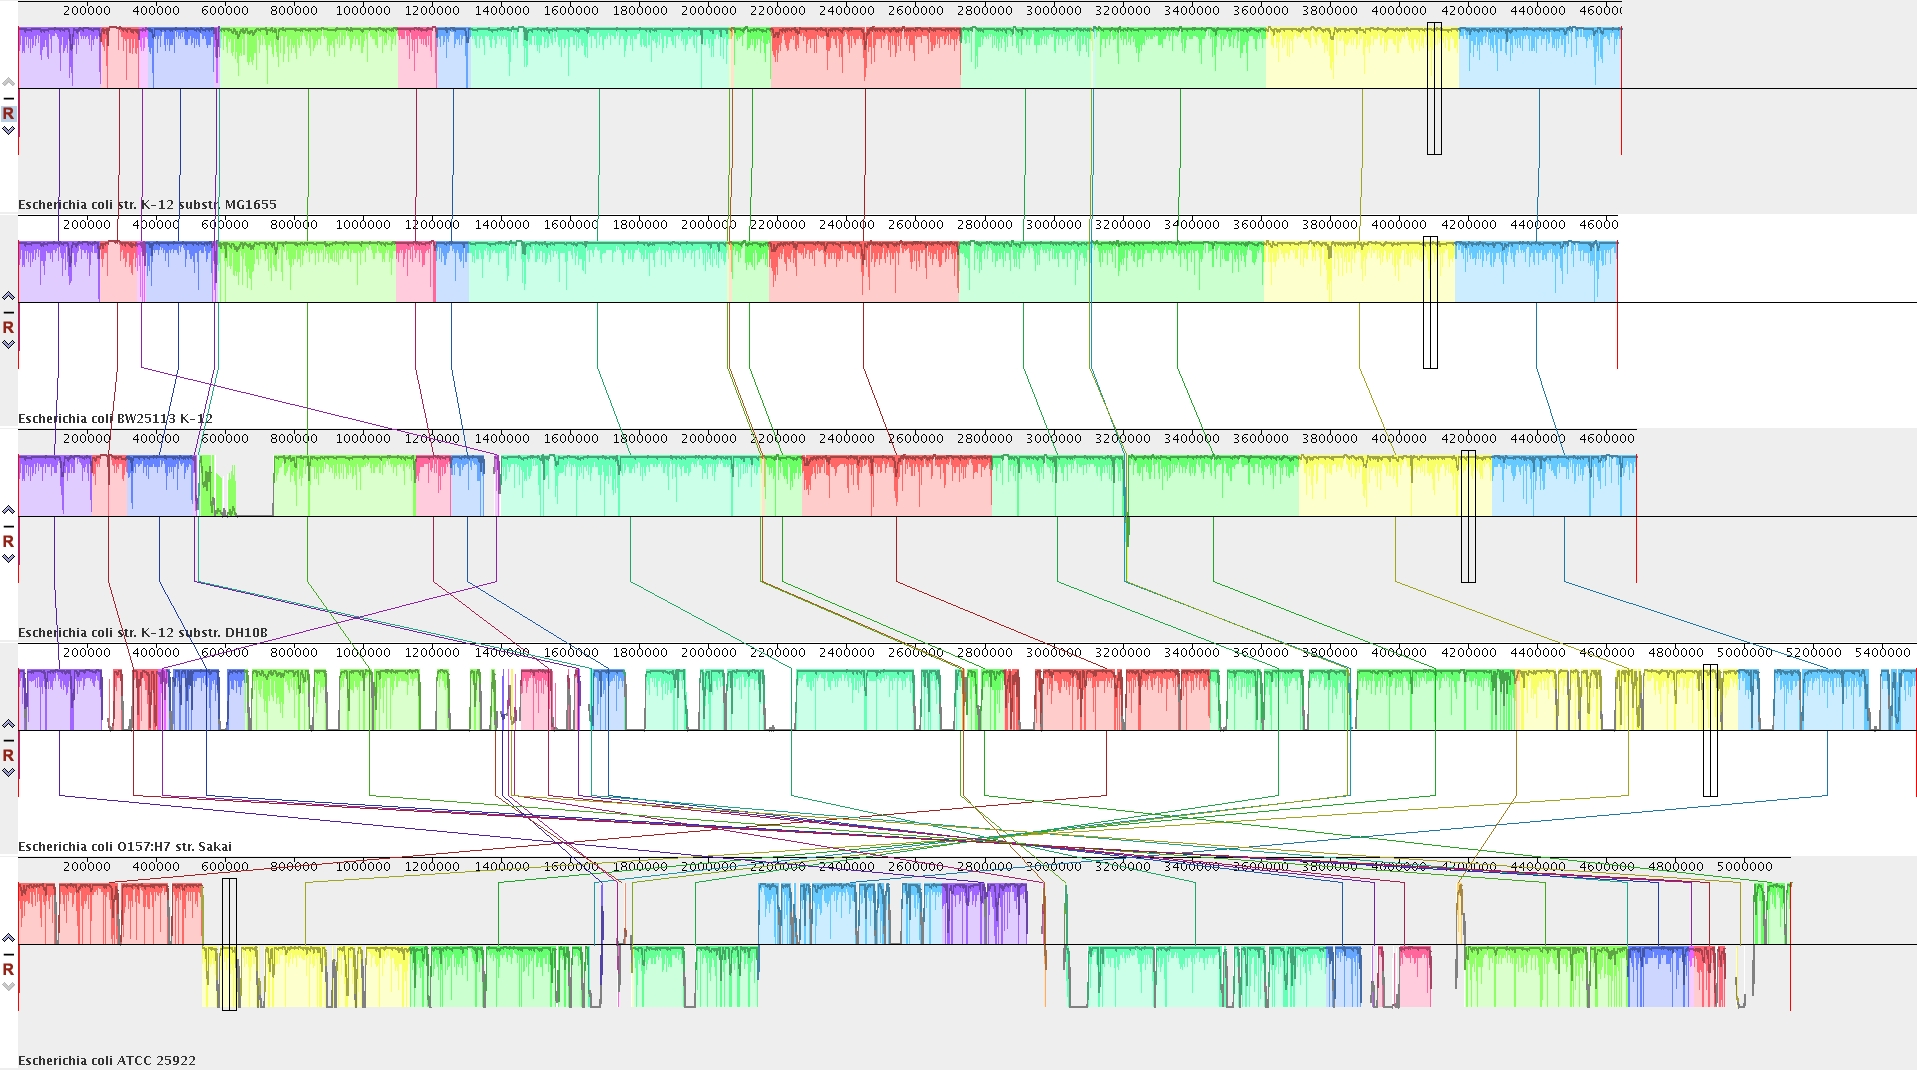
\includegraphics[width=\textwidth]{Mauve_aln_pic_17Dec18.jpg}
%%
%%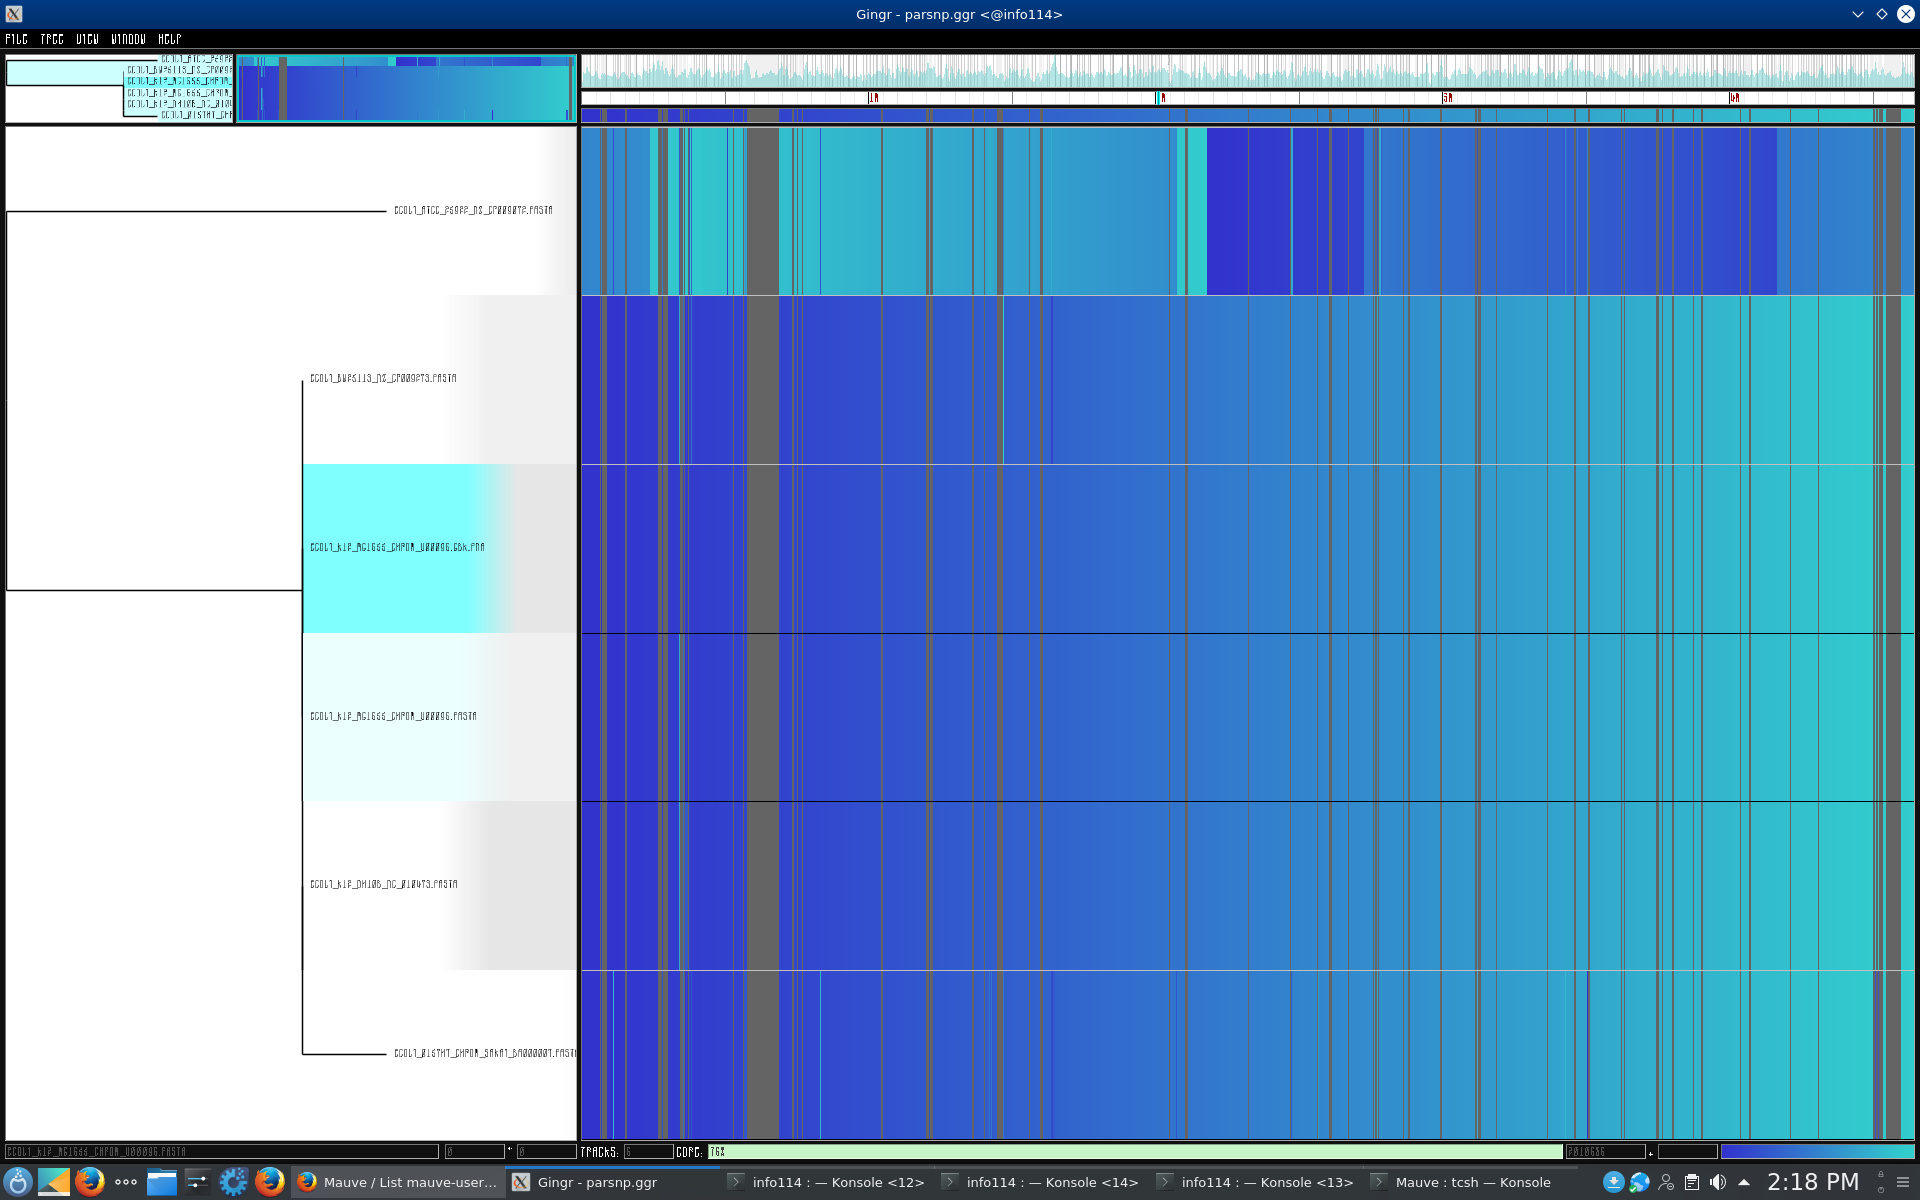
\includegraphics[width=\textwidth]{Parsnp_aln_pic_17Dec18.png}
%%
%
%%\begin{table}[h]
%%	\centering
%%	\resizebox{\textwidth}{!}{%
%%		\begin{tabular}{lccrr}
%%			\toprule
%%			Bacteria and Replicon & \% of Coding Sequences & \% of Non-Coding Sequences & \% of Subs Coding & \% of Subs Non-Coding\\
%%			\midrule
%%			\ecol Chromosome & 86.47\% & 13.53\% & 5.00\% & 8.96\% \\ % 4013445/4641652 & 200860 & 56265 
%%			\bass Chromosome & 87.49\% & 12.51\% & 7.31\% & 6.42\%\\ %3688210/4215606 & 269482 & 33846
%%			\strep Chromosome & 89.03\% & 10.97\% & 13.74\% & 14.91\%\\ % 7716382/8667507 & 1060278 & 141828
%%			\smel Chromosome & 86.27\% & 13.73\% & 0.19\% & 0.22\%\\ % 3152315/3654135 & 6023 & 1088
%%			\smel pSymA & 83.34\% & 16.66\% & 2.84\% & 4.58\%\\ % 1128615/1354226 & 225611/1354226 & 32040 & 10333
%%			\smel pSymB & 88.81\% & 11.19\% & 2.78\% & 3.44\%\\ % 1495047/1683333 & 41532 & 6483
%%			\bottomrule
%%		\end{tabular}
%%		
%%	}%resizebox
%%	\caption{\label{tab:cod_non_cod_proportions} Total proportion of coding and non-coding sites in each replicon and the percentage of those sites that have a substitution (multiple substitutions at one site are counted as two substitutions).}
%%\end{table}
%
%%
%%
%
%%
%%
%%\begin{table}[h]
%%	\centering
%%	\resizebox{\textwidth}{!}{%
%%		\begin{tabular}{lccc}
%%			\toprule
%%			Bacteria and Replicon & Coefficient Estimate & Standard Error & P-value \\
%%			\midrule
%%			\ecol Chromosome & 2.496\e{-5} & 8.695\e{-6}& 0.0041 \\
%%			\bass Chromosome & 1.912\e{-6} & 8.753
%%			\e{-8} & $<$2\e{-16}\\
%%			\strep Chromosome & 2.984\e{-5} & 1.858\e{-6} & $<$2\e{-16}\\
%%			\smel Chromosome & 6.993\e{-6} & 6.205\e{-7} & $<$2\e{-16}\\
%%			\smel pSymA & -9.713\e{-7} & 3.212\e{-8} & $<$2\e{-16}\\
%%			\smel pSymB & 6.181\e{-7} & 2.253\e{-8} & $<$2\e{-16}\\
%%			\bottomrule
%%		\end{tabular}
%%		
%%	}%resizebox
%%	\caption{\label{tab:cod_log_reg} Logistic regression analysis of the number of substitutions along all coding portions of the genome of the respective bacteria replicons. Grey coloured boxes indicate a negative logistic regression coefficient estimate. All results are statistically significant. Logistic regression was calculated after the origin of replication was moved to the beginning of the genome and all subsequent positions were scaled around the origin accounting for bidirectionality of replication.}
%%\end{table}
%%
%%\begin{table}[h]
%%	\centering
%%	\resizebox{\textwidth}{!}{%
%%		\begin{tabular}{lccc}
%%			\toprule
%%			Bacteria and Replicon & Coefficient Estimate & Standard Error & P-value \\
%%			\midrule
%%			\ecol Chromosome & -1.397\e{-7} & 2.427\e{-9} & $<$ 2\e{-16} \\
%%			\bass Chromosome & -1.439\e{-8} & 1.569\e{-9} & $<$2\e{-16}\\
%%			\strep Chromosome & 1.689\e{-8} & 7.235\e{-10} & $<$2\e{-16}\\
%%			\smel Chromosome & -1.311\e{-6}& 3.393\e{-8}& $<$2\e{-16}\\
%%			\smel pSymA & -1.413\e{-7} & 3.762\e{-8} & 1.73\e{-4}\\
%%			\smel pSymB & 5.196\e{-7} & 4.769\e{-8} & $<$2\e{-16}\\
%%			\bottomrule
%%		\end{tabular}
%%		
%%	}%resizebox
%%	\caption{\label{tab:non_cod_log_reg} Logistic regression analysis of the number of substitutions along all non-coding portions of the genome of the respective bacteria replicons. Grey coloured boxes indicate a negative logistic regression coefficient estimate. All results are statistically significant. Logistic regression was calculated after the origin of replication was moved to the beginning of the genome and all subsequent positions were scaled around the origin accounting for bidirectionality of replication.}
%%\end{table}
%
%\begin{table}[h]
%	\centering
%	\resizebox{0.8\textwidth}{!}{\begin{minipage}{\textwidth}
%			\begin{tabular}{lll}
%				\toprule
%				Bacteria Strain/Species & GEO Accession Number & Date Accessed\\
%				\midrule
%				\ecol K12 MG1655  & GSE60522 & December 20, 2017\\
%				\ecol K12 MG1655 & GSE73673 & December 19, 2017\\
%				\ecol K12 MG1655 & GSE85914 & December 19, 2017\\
%				\ecol K12 MG1655 & GSE40313 & November 21, 2018\\
%				\ecol K12 MG1655 & GSE114917 & November 22, 2018\\
%				\ecol K12 MG1655 & GSE54199 & November 26, 2018\\
%				\ecol K12 DH10B & GSE98890 & December 19, 2017\\
%				\ecol BW25113 & GSE73673 & December 19, 2017 \\
%				\ecol BW25113 & GSE85914 & December 19, 2017 \\
%				\ecol O157:H7 & GSE46120 & August 28, 2018\\
%				\ecol ATCC 25922 & GSE94978 & November 23, 2018\\
%% ecoli has lots of aerobic anerobic...etc growth phases, and time periods
%				\midrule
%				\bass 168 & GSE104816 & December 14, 2017\\
%				\bass 168 & GSE67058 & December 16, 2017\\
%				\bass 168 & GSE93894 & December 15, 2017\\
%				\bass 168 & GSE80786 & November 16, 2018\\
%				% bass also has quite a few time dependent data sets, or separated by growth phase				
%				\midrule
%				\scoe A3 & GSE57268 & March 16, 2018\\
%				\snat HW-2 & GSE112559 & November 15, 2018\\
%				% strep has LOTS of time dependent data sets, but the other bac do not really have that				
%				\midrule
%				\smel 1021 Chromosome & GSE69880 & December 12, 2017\\
%				%				\smel 1021 Chromosome & GSE121228 & diff phases\\
%				\midrule
%				\smel 2011 \pa & NC\_020527 (Dr. Finan) & April 4, 2018 \\
%				\smel 1021 \pa & GSE69880 & November 15, 18\\
%				\midrule
%				\smel 2011 \pb & NC\_020560 (Dr. Finan) & April 4, 2018 \\
%				\smel 1021 \pb & GSE69880 & November 15, 18\\
%				\bottomrule
%				
%				
%			\end{tabular}
%			\caption{\label{tab:tableS1} Summary of strains and species found for each gene expression analysis. Gene Expression Omnibus accession numbers and date accessed are provided.}
%		\end{minipage}}
%	\end{table}	
%
%
%
%
%
%%\begin{table}[]
%%	\centering
%%	\resizebox{\textwidth}{!}{%
%%		\begin{tabular}{lcccccc}
%%			\toprule
%%			Position Difference & \ecol Chromosome &\bass Chromosome & \strep Chromosome & \smel Chromosome &\smel pSymA & \smel pSymB\\
%%	\midrule
%%	1bp & -1.394\e{-7}** & -2.538\e{-8}** & 1.736\e{-8}** & -1.541\e{-6}** & -9.130\e{-7}** & 2.488\e{-7}*** \\
%%	10bp & -1.394\e{-7}*** & -2.518\e{-8}*** & -4.484\e{-9}*** & -1.627\e{-6}*** & -9.13\e{-7}*** & 3.487\e{-7}***\\
%%	100bp & -1.764\e{-7}*** & -1.417\e{-8}*** & 1.448\e{-8}*** & -1.605\e{-6}*** & -1.166\e{-6}*** & 4.021\e{-7}*** \\
%%	1000bp & -1.784\e{-7}*** & -1.417\e{-8}*** & 1.505\e{-8}*** & -1.605\e{-6}*** & -1.153\e{-6}*** & 4.021\e{-7}***\\
%%	10000bp & -1.712\e{-7}*** & -3.496\e{-8}*** & 4.790\e{-8}*** & -1.605\e{-6}*** & -3.570\e{-8}* & 3.784\e{-7}*** \\
%%	100000bp & -2.061\e{-7}*** & -3.561\e{-8}*** & 4.167\e{-9}*** & -1.605\e{-6}*** & -4.676\e{-7}*** & 3.784\e{-7}***\\
%%	1000000bp & 4.229\e{-8}*** & -7.710\e{-9}*** & 6.083\e{-8}*** &-1.605\e{-6}*** & 4.285\e{-6}*** & -8.888\e{-7}*** \\
%%	\bottomrule
%%		\end{tabular}
%%		
%%	}%resizebox
%%	\caption{\label{tab:clustering} Position clustering analysis. Logistic regression analysis of the number of substitutions along the genome of the respective bacteria replicons to test position differences. Each row denotes different base pair distances that the positions were clustered together as. All results are marked with significance codes as followed: $<$ 0.001 = `***', 0.001 $<$ 0.01 = `**', 0.01 $<$ 0.05 = `*', 0.05 $<$ 0.1 = `.', $>$ 0.1 = ` '. Logistic regression was calculated after the positions in the genome were determined to be the same at each position difference listed in the first column.}
%%\end{table}
%%
%%
%
%
%%\begin{table}[b!]
%%	\centering
%%	\resizebox{\textwidth}{!}{%
%%		\begin{tabular}{lccc}
%%			\toprule
%%			Bacteria and Replicon & Coefficient Estimate & Standard Error & P-value \\
%%			\midrule
%%			\cellcolor{black!16}\ecol Chromosome & \cellcolor{black!16}-1.394\e{-7} & \cellcolor{black!16}2.425\e{-9} & \cellcolor{black!16}$<$2\e{-16} \\
%%			\cellcolor{black!16}\bass Chromosome & \cellcolor{black!16}-1.265\e{-8} & \cellcolor{black!16}1.562\e{-9} & \cellcolor{black!16}5.430\e{-16} \\
%%			\strep Chromosome & 1.736\e{-8} & 7.231\e{-10} & $<$2\e{-16}\\
%%			\cellcolor{black!16}\smel Chromosome & \cellcolor{black!16}-1.541\e{-6} & \cellcolor{black!16}3.042\e{-8} & \cellcolor{black!16}$<$2\e{-16}\\
%%			\cellcolor{black!16}\smel pSymA & \cellcolor{black!16}-9.130\e{-7} & \cellcolor{black!16}1.975\e{-8} & \cellcolor{black!16}$<$2\e{-16} \\
%%			\smel pSymB & 2.488\e{-7} & 1.964\e{-8} & $<$2\e{-16}\\
%%			\bottomrule
%%		\end{tabular}
%%		
%%	}%resizebox
%%	\caption{\label{tab:tabel2} Logistic regression analysis of the number of substitutions along the genome of the respective bacteria replicons. Grey coloured boxes indicate a negative logistic regression coefficient estimate. All results are statistically significant. Logistic regression was calculated after the origin of replication was moved to the beginning of the genome and all subsequent positions were scaled around the origin accounting for bidirectionality of replication.}
%%\end{table}
%%
%%
%%
%%\includegraphics[width=\textwidth]{C:/Users/Daniella/Documents/Sinorhizobium2015/Gene_Expression_8Dec17/Gene_Expression/smel_chrom_sub_exp_histogram_bidirectionality_colour_16Mar18}
%%
%%\includegraphics[width=\textwidth]{C:/Users/Daniella/Documents/Sinorhizobium2015/Gene_Expression_8Dec17/Gene_Expression/pSymA_sub_exp_histogram_bidirectionality_colour_9Apr18}
%%
%%\includegraphics[width=\textwidth]{C:/Users/Daniella/Documents/Sinorhizobium2015/Gene_Expression_8Dec17/Gene_Expression/pSymB_sub_exp_histogram_bidirectionality_colour_12Apr18}
%%
%%\includegraphics[width=\textwidth]{C:/Users/Daniella/Documents/Sinorhizobium2015/Gene_Expression_8Dec17/Gene_Expression/bass_chrom_sub_exp_histogram_bidirectionality_colour_5Apr18}
%%
%%\includegraphics[width=\textwidth]{C:/Users/Daniella/Documents/Sinorhizobium2015/Gene_Expression_8Dec17/Gene_Expression/ecoli_chrom_sub_exp_histogram_bidirectionality_colour_16Mar18}
%%
%%\includegraphics[width=\textwidth]{C:/Users/Daniella/Documents/Sinorhizobium2015/Gene_Expression_8Dec17/Gene_Expression/strep_chrom_sub_exp_histogram_bidirectionality_colour_19Mar18}
%%
%%%\begin{table}[h]
%%%	\centering
%%%	\resizebox{\textwidth}{!}{%
%%%		\begin{tabular}{lccc}
%%%			\toprule
%%%			Bacteria and Replicon & Coefficient Estimate & Standard Error & P-value \\
%%%			\midrule
%%%			\ecol Chromosome & -1.44\e{-7}& 2.01\e{-9} & $<$2\e{-16}\\
%%%			\bass Chromosome & -1.121\e{-7} & 3.41\e{-9} & $<$2\e{-16}\\
%%%			\strep Chromosome & 1.24\e{-8} & 7.2\e{-10} & $<$2\e{-16}\\
%%%			\smel Chromosome & -1.526\e{-6} & 3.02\e{-8} & $<$2\e{-16}\\
%%%			\smel pSymA & -1.058\e{-6}& 2.58\e{-8}& $<$2\e{-16}\\
%%%			\smel pSymB & 1.79\e{-7}& 1.84\e{-8}& 1.6\e{-10}\\
%%%			\bottomrule
%%%		\end{tabular}
%%%		
%%%	}%resizebox
%%%	\caption{\label{tab:tabel2} Logistic regression analysis of the number of substitutions along the genome of the respective bacteria replicons when 10,000bp sections of the genome are re-organized.}
%%%\end{table}
%%
%%
%%\begin{table}[]
%%	\centering
%%	\resizebox{1.2\textwidth}{!}{%
%%			\begin{tabular}{lcccccc}
%%\toprule
%%Origin Location & \ecol Chromosome &\bass Chromosome & \strep Chromosome & \smel Chromosome &\smel pSymA & \smel pSymB\\
%%\midrule
%%Moved 100kb Left & -1.445\e{-7}*** & 4.374\e{-9}* &  6.909\e{-9}*** &  -1.316\e{-6}*** & -1.058\e{-6}*** & -2.009\e{-7}***\\
%%Moved 90kb Left & -1.544\e{-7}*** & -1.036\e{-7}*** & 5.677\e{-9}*** & -1.32\e{-6}*** & -1.246\e{-6}*** &-1.357\e{-7}***\\
%%Moved 80kb Left& -1.65\e{-7}*** & -1.072\e{-7}*** & 8.11\e{-9}*** & -1.338\e{-6}*** & -1.398\e{-6}*** & -6.57\e{-8}***\\
%%Moved 70kb Left& -1.667\e{-7}*** & -1.102\e{-7}*** & 6.716\e{-9}*** & -1.363\e{-6}*** & -1.405\e{-6}*** & 9.83\e{-8}\\
%%Moved 60kb Left& -1.64\e{-7}*** & -1.19\e{-7}*** & 8.7\e{-9}*** & -1.324\e{-6}*** & -1.394\e{-6}*** & 1.129\e{-7}***\\
%%Moved 50kb Left& -1.446\e{-7}*** & -1.211\e{-7}*** & 1.045\e{-8}*** & -1.36\e{-6}*** & -1.403\e{-6}*** & 1.521\e{-7}***\\
%%Moved 40kb Left& -1.4\e{-7}*** & -1.299\e{-7}*** & 1.214\e{-8}*** & -1.255\e{-6}*** & -1.422\e{-6}*** & 1.543\e{-7}***\\
%%Moved 30kb Left& -1.498\e{-7}*** & -1.292\e{-7}*** & 1.24\e{-8}*** & -1.26\e{-6}*** & -1.392\e{-6}*** & 1.63\e{-7}***\\
%%Moved 20kb Left& -1.51\e{-7}*** & -1.1\e{-7}*** & 1.395\e{-8}*** & -1.525\e{-6}*** & -1.412\e{-6}*** & 1.603\e{-7}***\\
%%Moved 10kb Left& -1.262\e{-7}*** & -2.602\e{-9} & 1.563\e{-8}*** &  -1.599\e{-6}*** &  -9.499\e{-7}*** & 2.973\e{-7}*** \\
%%Moved 10kb Right& -1.305\e{-7}*** & -2.045\e{-8}*** & 1.578\e{-8}*** & 1.614\e{-6}*** & -1.026\e{-6}*** & 3.505\e{-7}*** \\
%%Moved 20kb Right& -1.454\e{-7}*** & -1.006\e{-7}*** & 1.903\e{-8}*** & -1.634\e{-6}*** & -1.475\e{-6}*** & 1.649\e{-7}***\\
%%Moved 30kb Right& -1.548\e{-7}*** & -8.596\e{-8}*** & 2.046\e{-8}*** & -1.698\e{-6}*** & -1.417\e{-6}*** & 1.526\e{-7}***\\
%%Moved 40kb Right& -1.632\e{-7}*** & -8.378\e{-8}*** & 2.125\e{-8}*** & -1.719\e{-6}*** & -1.367\e{-6}*** & 1.589\e{-7}***\\
%%Moved 50kb Right& -1.856\e{-7}*** & -7.879\e{-8}*** & 1.957\e{-8}*** & -1.735\e{-6}*** & -1.277\e{-6}*** & 1.654\e{-7}***\\
%%Moved 60kb Right& -1.91\e{-7}*** & -6.98\e{-8}*** & 1.974\e{-8}*** & -1.788\e{-6}*** & -1.169\e{-6}*** & 1.645\e{-7}***\\
%%Moved 70kb Right& -1.892\e{-7}*** & -6.634\e{-8}*** & 1.934\e{-8}*** & -1.854\e{-6}*** & -1.059\e{-6}*** & 1.843\e{-7}***\\
%%Moved 80kb Right& -1.879\e{-7}** & -5.814\e{-8}*** & 2.313\e{-8}*** & -1.891\e{-6}*** & -9.07\e{-7}*** & 1.90\e{-7}***\\
%%Moved 90kb Right& -1.862\e{-7}*** & -4.314\e{-8}*** & 2.304\e{-8}*** & -1.865\e{-6}*** & -7.171\e{-7}*** & 2.415\e{-7}***\\
%%Moved 100kb Right& -1.799\e{-7}*** & -2.597\e{-8}*** &  1.945\e{-8}*** &  -1.525\e{-6}*** & -6.572\e{-7}*** & 3.095\e{-7}***\\
%%\bottomrule
%%\end{tabular}
%%		
%%	}%resizebox
%%	\caption{\label{tab:tabel2} Logistic regression analysis of the number of substitutions along the genome of the respective bacteria replicons. All results are marked with significance codes as followed: $<$ 0.001 = `***', 0.001 $<$ 0.01 = `**', 0.01 $<$ 0.05 = `*', 0.05 $<$ 0.1 = `.', $>$ 0.1 = ` '. Logistic regression was calculated after the origin of replication was moved to the beginning of the genome and all subsequent positions were scaled around the origin accounting for bidirectionality of replication.}
%%\end{table}
%%
%%%\begin{table}[h]
%%%	\resizebox{\textwidth}{!}{%
%%%		\begin{tabular}{lccc}
%%%			\toprule
%%%			Bacteria Replicon & \multicolumn{1}{p{3cm}}{\centering \% of Total LCBs \\ with Identical Tree} & 
%%%			\multicolumn{1}{p{3cm}}{\centering \% of Total LCBs \\ with Not Identical Tree} & 
%%%			\multicolumn{1}{p{3cm}}{\centering \% of Total Alignment Discarded} \\  
%%%			\midrule
%%%			\ecol Chromosome & 81.58\% & 18.42\% & 25.18\%\\
%%%			\bass Chromosome & 83.33\% & 16.67\% & 19.37\%\\
%%%			\strep Chromosome & 96.53\% & 3.47\% & 12.42\%\\
%%%			\smel Chromosome & 81.82\% & 18.18\% & 25.42\%\\
%%%			\smel \pa & 100\% & 0\% & 0\%\\
%%%			\smel \pb & 100\% & 0\% & 0\%\\
%%%			\bottomrule
%%%		\end{tabular}
%%%	}%resize box
%%%\end{table}
%%%
%%% 
%%
%%%
%%%\clearpage
%%%
%%%
%%%
\end{document}
